% !TeX root = ../libro.tex
% !TeX encoding = utf8

\chapter{Rotación y campos magnéticos de intensidad variable}\label{ch:sexto-capitulo}

\section{Introducción}
--ELABORAR LA INTRODUCCIÓN. REVISAR PAPER2--
Suponer que la intensidad del campo magnético de una estrella permanece constante a lo largo de su evolución es una simplificación necesaria en algunos escenarios, pero no se corresponde con las observaciones (INDICAR LAS REFERENCIAS). \par

--EXPLICAR POR QUÉ OPTAMOS POR LA INTENSIDAD VARIABLE
La segunda línea de trabajo se encaminó a extender MESA para que soportara la influencia de campos magnéticos y $\amlt$ variable en la evolución de su estrella anfitriona.
Adicionalmente a lo de la parte 1
\begin{itemize}
	\item Presencia de campo magnético de intensidad variable
	\item Evolución temporal de $\amlt$
\end{itemize}
\section{Efectos del frenado magnético - Parte II}

\subsection{Formalismo de frenado magnético de intesidad variable} 
De acuerdo a \cite{Gallet2013} la intensidad del campo magnético debería variar a lo largo de la vida de la estrella en lugar de permanecer fija durante toda su evolución. Para ello nos basamos en un formalismo que nos permite calcular una intensidad de campo magnético variable. 

\subsubsection{Frenado magnético según Gallet \& Bouvier (2013)}
Este modelo adopta una prescripción de tipo dinamo que permite establecer una relación entre $\Omega$ , $\teff$, y la intensidad del campo magnético ($B$), así como con la tasa de pérdida de masa ($\mwind$) causada por el viento estelar. Comenzaremos enumerando los aspectos más relevantes y las suposiciones realizadas en la modelización de la evolución de la intensidad del campo magnético.\par 

Un parámetro relevante para caracterizar la influencia de un campo magnético dado en el viento estelar es $\Omega$. Suponiendo que el campo magnético es generado por una dinamo, su fuerza es proporcional a alguna potencia de $\Omega$,

\begin{equation}
	f_*B_* \propto \Omega_*^b \label{eq:mf_strenght}
\end{equation}

donde $f_*$ es el factor de llenado, es decir, la fracción de la superficie estelar que está magnetizada, $B_*$ es la fuerza del campo magnético, $\Omega_*$ es la velocidad angular de la estrella en la superficie estelar, y $b$ es el exponente de la dinamo \citep{Gallet2013}. El producto de $f_*$ por $B_*$ nos permitirá obtener la intensidad del campo magnético. \par

Según este enfoque, la intensidad del campo magnético variará proporcionalmente a la temperatura efectiva ($\teff$) de la estrella de la siguiente manera: 
\begin{ceqn}
	\begin{equation}
		B_* \approx 1.13 \Beq \label{eq:mf_bstar}
	\end{equation}
\end{ceqn}

donde $B_*$ es proporcional a la intensidad del campo magnético de equipartición, quedando $\Beq$ definido como 

\begin{equation}
	\Beq = \sqrt{8\pi P_*} = \sqrt{\frac{8\pi\rho_* \boltzmann \teff}{\mu\massH}}\label{eq:mf_beq}    
\end{equation}

donde $P_*$ es la presión del gas fotosférico, $\rho_*$ es la densidad fotosférica, $\boltzmann$ es la constante de Boltzmann, $\massH$ es la masa de un átomo de hidrógeno, y $\mu$ el peso atómico medio \citep{Cranmer2011}. \par

Como se indica en \cite{Cranmer2011} $\mu$ puede estimarse utilizando las ecuaciones de estado del plasma OPAL \footnote{\url{https://opalopacity.llnl.gov/EOS_2005/}},

\begin{equation}
	\mu \approx \frac{7}{4} + \frac{1}{2} \; \textrm{tanh}\Bigg(\frac{3500-\teff}{600}\;\Bigg) \label{eq:mf_atom_weight}
\end{equation}

Finalmente, estamos en condiciones de calcular $\Beq$ y $B_*$.\par

Por otro lado, \cite{Cranmer2011} descubrió que la intensidad del campo magnético está influida principalmente por $f_*$ y no por el periodo de rotación de la estrella. Es decir, las variaciones en la velocidad angular de la estrella no alteran significativamente la intensidad de su campo magnético. Además, $f_*$ depende en gran medida del número de Rossby ($\rossby$). Para calcular $\rossby$ de una estrella determinada, es necesario conocer el tiempo de vuelta ($\turnover$),

\begin{equation}
	\rossby = \frac{\prot}{\turnover} \label{eq:mf_rossby}
\end{equation}
\begin{equation}
	\turnover = 314.24\;exp\left[-\Bigg(\frac{\teff}{1952.5}\Bigg)-\Bigg(\frac{\teff}{6250}\Bigg)^{18} \;\right]+0.002 \label{eq:mf_turnover}
\end{equation}

\cite{Cranmer2011} proporciona dos ajustes diferentes para $f_*$ que definen respectivamente los límites superior e inferior para la intensidad media del campo magnético superficial ($f_*B_*$),

\begin{align}
	\fmin &= \frac{0.5}{(1+(x/0.16)^{2.6})^{1.3}} \label{eq:fmin}\\
	\fmax &= \frac{1}{1+(x/0.31)^{2.5}} \label{eq:fmax}
\end{align}

donde x = $\rossby$/$\rossbysun$, y $\rossbysun$ = 1.96. \par

Por último, podemos calcular el factor de llenado de una estrella aplicando el ajuste realizado por \cite{Gallet2013} que reproduce más fielmente el factor de llenado medio del Sol actual ($\fsun$ = [0.001-0.01], ver \citep{Cranmer2011}),


\begin{figure}
	\centering
	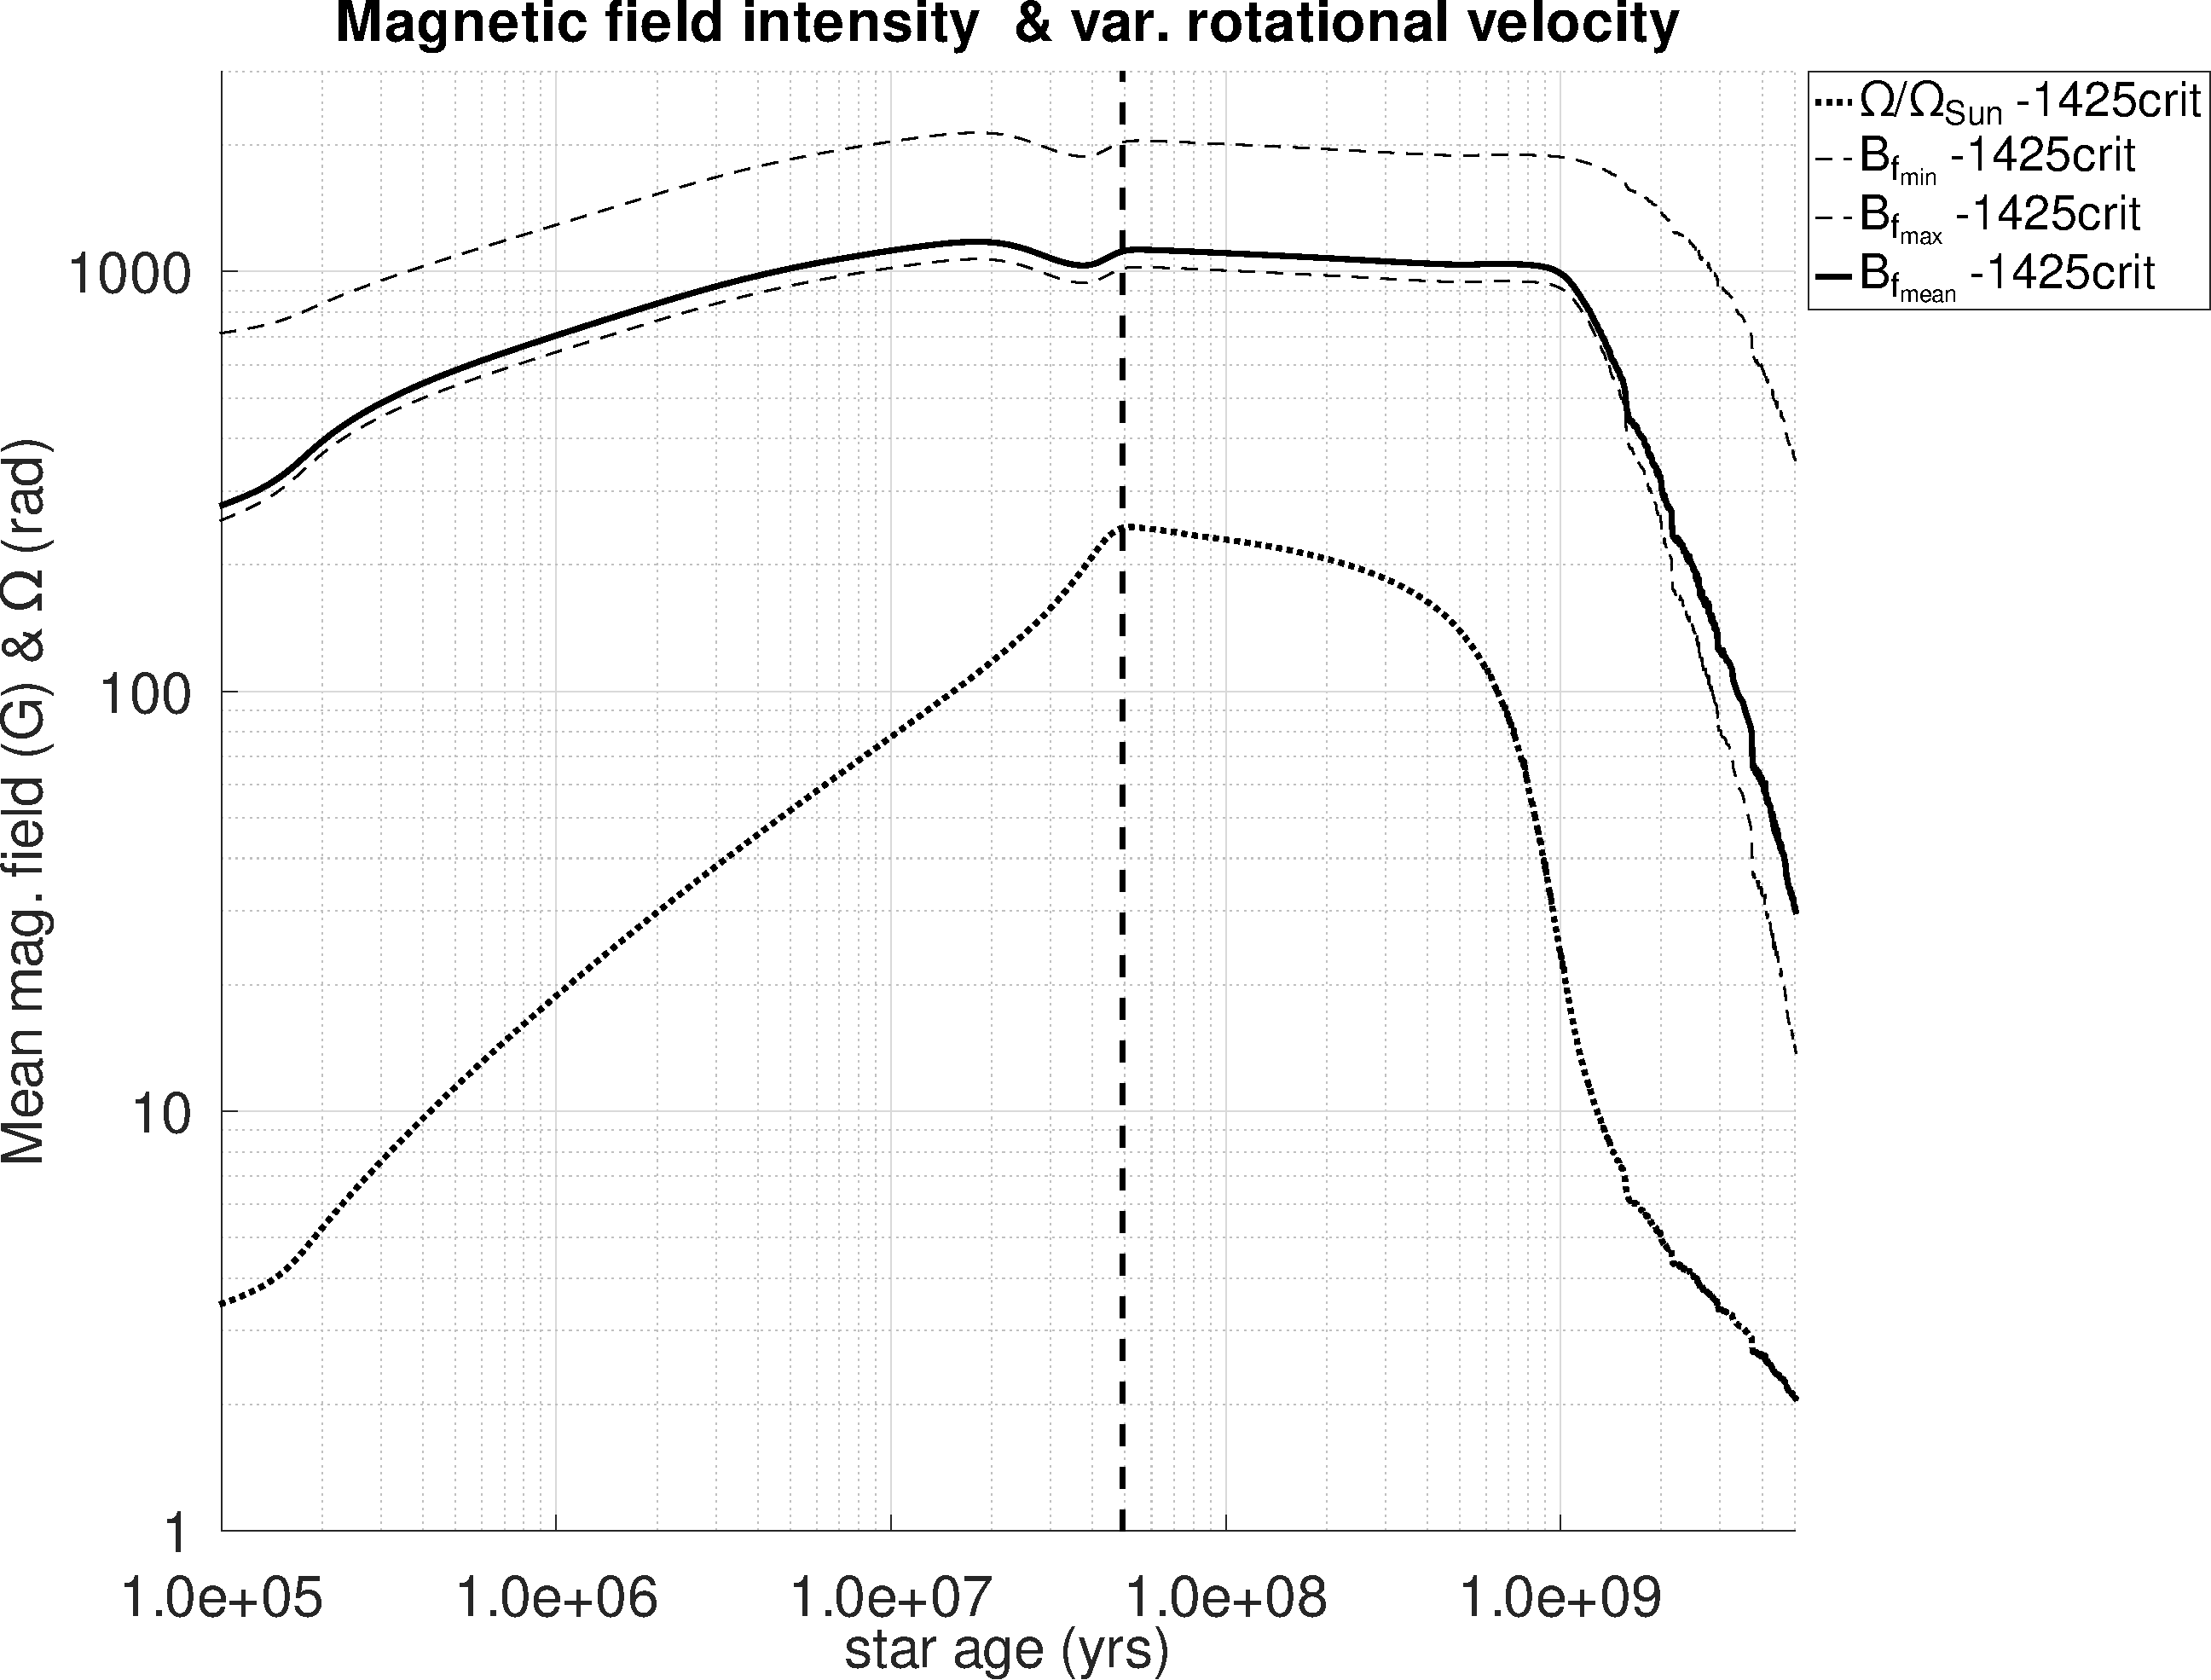
\includegraphics[width=0.5\textwidth]{img/paper2/mag_field_limits_var_vel_g3.pdf}
	\caption{La evolución de la intensidad del campo magnético y sus límites superior e inferior, en función del tiempo y $\oomegac$ para varios modelos de 1 $\msun$. El modelo incluye rotación PMS con $\oomegac$ = 0.1425. Las líneas continuas representan la intensidad del campo magnético, mientras que las líneas discontinuas representan la evolución angular de la estrella. La línea vertical discontinua hace referencia a la ZAMS.}
	\label{fig:mag_field_limits_var_vel_g3}
\end{figure}

Con este formalismo podemos calcular el campo magnético medio como una función dependiente del tiempo, de $\rho$, $\teff$, y $\Omega$. Los valores temporales de estas tres variables se obtendrán a partir de las distintas simulaciones realizadas con ayuda de MESA. \par


--QUIZAS SACARLO A UNA SECCIÓN PROPIA DE AML --
Una vez que hemos caracterizado cómo evoluciona la intensidad del campo magnético, necesitamos modelar cómo se produce la pérdida de momento angular. A medida que la estrella se contrae durante la fase de PMS hacia el comienzo de la ZAMS, su velocidad angular aumenta, lo que conduce a un aumento gradual del campo magnético medio. En nuestro análisis, observamos intensidades máximas de hasta $1.0,\mathrm{kG}$, como se muestra en la figura \ref{fig:mag_field_limits_var_vel_g3}. A continuación, entra en una fase de saturación (aunque con una tendencia descendente) hasta $1.0$ Ga, y finalmente disminuye bruscamente como resultado de la menor velocidad angular de la estrella. En el formalismo anterior utilizamos un modelo aplicable a campos magnéticos de intensidad no variable y de baja intensidad que oscilan entre unos pocos Gauss ($1.0,\mathrm{G} \leq B \leq 10.0,\mathrm{G}$). Las intensidades significativamente mayores requeridas en el presente formalismo hacen inadecuado el modelo empleado anteriormente.\par


Comencemos por enumerar los aspectos más relevantes y las suposiciones realizadas en la modelización de la evolución de la rotación, el frenado magnético y el momento angular. Si suponemos un flujo de salida esférico, el par aplicado por un viento estelar $\torquewind$ acoplado magnéticamente viene dictado por,

\begin{equation}
	\torquewind \propto \Omega_* \; \mwind \; \ralfven^{2} \label{eq:mb_torque}
\end{equation}

donde $\mwind$ es la tasa de pérdida de masa, y $\ralfven$ el valor medio del radio de Alfvén. \par

Las estrellas con masas iniciales similares, pero con diferentes ratios de pérdida de masa ($\Dot{M}$), acabarán evolucionando de forma muy diferente. Las partículas ionizadas transportadas por el viento solar no sólo contribuyen a la pérdida de masa, sino también a la pérdida de energía cinética que se deposita en el medio interestelar. Dada una estrella con un viento esféricamente simétrico, $\mwind$ se caracteriza por la siguiente expresión:

\begin{ceqn}
	\begin{equation}
		\mwind = 4\pi r^2\rho\nu \label{eq:mass_loss}
	\end{equation}
\end{ceqn}

donde $r$ es el radio estelar, $\rho$ la densidad de masa, y $\nu$ la velocidad del viento estelar.

--BLOQUE REPETIDO. HACER REFERENCIA A LA SECCIÓN ANTERIOR, INDICANDO QUE A DIFERENCIA DE ELLA, AQUÍ UTILIZAMOS R-ALVEN--
Se ha observado que las estrellas de masa intermedia fuertemente magnéticas suelen tener tasas de rotación mucho más lentas que otras estrellas de su población parental \cite{Mathys2006}. En esas estrellas, los campos magnéticos interactúan con la pérdida de masa, donde el radio Alfv'{e}n juega un papel importante. $\ralfven$ se define como el punto en el que la densidad de energía del campo magnético y la densidad de energía cinética están equilibradas. En caso de que $\ralfven$ sea mayor que el radio estelar, entonces el flujo del viento tendrá que seguir el campo magnético. Como consecuencia, el material abandona la superficie estelar con una mayor AM específica, ya que el radio de co-rotación ha aumentado y corresponde aproximadamente a $\ralfven$ que puede expresarse como \cite{Matt2012}

\begin{equation}
	\ralfven = K_1\left[\frac{\Bp^{2}\;R_*^{2}}{\mwind\;\sqrt{K_2^2\vesc^2 + \Omega_*^2R_*^{2}}\ }\right]^{m}R_*  \label{eq:mb_ralfven}
\end{equation}

donde $\Bp$ es la intensidad del campo magnético en la superficie estelar, $\vesc$ es la velocidad de escape, $m = 0.1675$, $K_1 = 1.30$ y $K_2 = 0.0506$ \citep{Gallet2013}.

\begin{align}
	\Bp &= f_*B_* \label{eq:bp}\\
	\vesc &= \sqrt{\frac{2\,G\,\mstar}{\rstar}} \label{eq:vesc}
\end{align}

Por último, tenemos que el AML puede calcularse del siguiente modo:

\begin{equation}
	\Dot{J} = \Omega_* \; \mwind \; \ralfven^{2} \label{eq:j_dot}
\end{equation}

donde $\mwind$ es la tasa de pérdida de masa. Esta expresión se implementa en MESA a partir de los valores expuestos directamente durante las simulaciones.

--HASTA AQUÍ--

\section{Efectos de la longitud de mezcla}
La teoría de la longitud de mezcla (Mixing Length Theory, MLT) introducida por \citet{BohmVit58} ha sido comúnmente adoptada para modelar la convección estelar en códigos de evolución estelar, incluyendo MESA. El parámetro libre más importante en esta teoría es la longitud de mezcla $l$ que se define como:

\begin{equation}
	l = \alpha H_p\label{eq:mixlength}
\end{equation}

donde $H_p$ es la altura de la escala de presión, y $\alpha$ un parámetro libre que se determina de antemano y se mantiene fijo durante las simulaciones de evolución estelar. \par

La influencia de los parámetros libres, relativamente arbitrarios, asociados a MLT condiciona significativamente la evolución de la abundancia de Li. Además, no existen argumentos sólidos que sugieran que el parámetro de longitud de mezcla sea el mismo en todas las estrellas y en todas las fases evolutivas \cite{Pasetto2014}. En la Sección \ref{sec:alt_mlt} mostramos cómo una parametrización alternativa de la longitud de mezcla (ML) podría producir resultados en línea con las observaciones. El ajuste del overshooting de ML y del parámetro libre $\amlt$ parece ser necesario para explicar las abundancias de litio en los OC's.\par

De manera similar a la intensidad del campo magnético, un formalismo que nos permita evolucionar a lo largo del tiempo el valor de $\amlt$ en función de determinados parámetros de la estrella, es un planteamiento razonable a la hora de eliminar una restricción relativamente arbitraria impuesta en nuestros modelos.

\subsection{MLT $\alpha$ variable según Sonoi et al. (2019)}
En \cite{Sonoi2018}, los autores introdujeron una forma de calibrar $\amlt$ para estrellas de tipo solar en la que su valor directamente proporcional a la $\gsurf$, e inversamente proporcional a la $\teff$. --CREAN UN SIMPLE EXCEL MOSTRANDO ESTO-- Calibraron diferentes valores de $\amlt$ para varios modelos 3D simulados usando el código CO$^5$BOLD \citep{Freytag2011} y los transfirieron a modelos 1D desarrollados por \cite{Ludwig1998}. La parametrización que obtuvieron fue: 

\begin{equation}
	f(x,y) = a_0 + (a_1 + (a_3 + a_5x +a_6y)x + a_4y)x + a_2y\label{eq:alpha_ml}
\end{equation}

donde

\begin{align}
	x &= \frac{\teff-5777}{1000} \label{eq:eq:alpha_x}\\
	y &= \gsurf-4.44 \label{eq:eq:alpha_y}
\end{align}

y $a_i$ son los coeficientes resultantes de la función de ajuste \ref{eq:alpha_ml} a los valores $\alpha$ calibrados para el modelo de convección MLT \citep{Sonoi2018}: $a_0=1.790295$, $a_1=-0.14954$, $a_2=0.069574$, $a_3=-0.00829$, $a_4=0.013165$, $a_5=0.080333$, $a_6=-0.03306$. \par
--COMENTAR MÁS EN DETALLE CÓMO, POR EJEMPLO, SE HACE VARIAR EN MESA. TAMBIÉN ALGO MÁS DEL FORMALISMO--



\section{Extendiendo MESA - Parte III}
\subsection{Rutina de frenado magnético de intensidad variable} \label{sec:mb_var_b}
En la Sección \ref{sec:mb_cte_b} comentamos los detalles de como MESA conserva el AM entre las diferentes celdas $k$ y les asigna un valor de AM $J_k$. Este mecanismo sigue siendo el mismo para esta nueva rutina. En este nuevo escenario la diferencia radica en la nueva rutina de MB (ver Listado \ref{lst:jdot_gb}), concretamente en la implementación de la misma según el nuevo formalismo que hemos introducido para campos magnéticos de intensidad variable, y especialmente en la rutina que calcula la intensidad del campo magnético, devolviendo (potencialmente) un valor diferente a cada paso de la simulación (ver Listado \ref{lst:jdot_mf_intensity}).\par

\begin{lstlisting}[language=Fortran, float, caption={Rutina de par de torsión para un campo magnético de intensidad variable.}, label={lst:jdot_gb}]
  real function calculate_jdot_rate_gb(s, bf_star) result(new_j_dot)
	use const_def
	type (star_info), pointer, intent(in) :: s
	real(dp), intent(in) :: bf_star
	real(dp), parameter :: k1 = 1.30
	real(dp), parameter :: k2 = 0.0506
	real(dp), parameter :: m = 0.1675
	real(dp), parameter :: omega_sun = 2.87d-6
	real(dp) :: r_st, m_st, omega_surf, j_dot
	real(dp) :: v_esc, m_dot, alfven_r, alfven_r_num, alfven_r_den
	
	!Star data
	r_st = s% r(1)
	m_st = s% m(1)
	omega_surf = s% omega(1)
	m_dot = abs(s% mstar_dot) !This in g/s
	
	v_esc = (2 * standard_cgrav * m_st / r_st)**0.5
	
	alfven_r_num = bf_star**2 * r_st**2
	alfven_r_den = m_dot*((k2**2 * v_esc**2)+(omega_surf**2 * r_st**2))**0.5
	alfven_r = k1 * (alfven_r_num / alfven_r_den)**m * r_st
	
	j_dot = omega_surf * m_dot * alfven_r**2
	
	new_j_dot = -j_dot
  end function	
\end{lstlisting}

\subsection{Rutina de cálculo de intensidad de campo magnético}
La incorporación del formalismo para calcular una intensidad de campo magnético variable representa una mejora sustancial al modelo presentado en el capítulo \ref{ch:tercer-capitulo}. Esta intensidad es funcionalmente dependiente del tiempo, de $\rho$, $\teff$, y $\Omega$, valores que podemos obtener directamente de MESA.\par

\begin{lstlisting}[language=Fortran, float, caption={Rutina de cálculo de intensidad de campo magnético.}, label={lst:jdot_mf_intensity}]
  real function calculate_mag_field_intensity_gb(s) result(new_b)
	use const_def
	type (star_info), pointer, intent(in) :: s
	
	! rossby_sun = 1.96, Eq 9 [1]
	real(dp) :: r_st, rossby_sun = 1.96, rossby, rossby_norm, m_hydrogen
	real(dp) :: p_rot, p_rot_sun = 25.38 !Carrington solar  rotation
	real(dp) :: tau_c_sun, tau_c, f_star, f_min, f_max, b_star
	real(dp) :: bf_min, bf_max, bf_star, b_equi, mu_avg
	real(dp) :: p_gas_photo, p_photo, p_rad_photo, p_photo2
	
	!tau_c -> convective turnover time (d)
	!exp ->  natural exponential function
	tau_c = 314.241*exp(-s% Teff/1952.5)*exp(-(s% Teff/6250)**18) + 0.002 
	tau_c_sun = 314.241*exp(-teffsun/1952.5)*exp(-(teffsun/6250)**18) + 0.002
	
	!Star data
	r_st = s% r(1)
	p_rot = (2*pi*r_st) / (s% v_rot_avg_surf * 86400) ! day
	
	!Rossby number = p_rot / tau_c
	rossby = p_rot / tau_c
	rossby_sun = p_rot_sun / tau_c_sun
	rossby_norm = rossby / rossby_sun
	
	!magnetic filling factor fmin & fmax
	f_min = 0.5 / (1. + (rossby_norm / 0.16)**2.6)**1.3 
	f_max = 1 / (1. + (rossby_norm / 0.31)**2.5)
	f_star = 0.55 / (1. + (rossby_norm / 0.16)**2.3)**1.22
	
	!Eq 3 [2]
	!mean atomic weight
	mu_avg = 1.75 + 0.5 * tanh((3500. - s% Teff) / 600.)
	!photospheric pressure 
	m_hydrogen = mp !proton mass       
	p_photo = s%rho(s% photosphere_cell_k)*boltzm*s% Teff/(mu_avg*m_hydrogen)
	!Equipartition magnetic filed strength
	b_equi = sqrt(8.* pi * p_photo)
	
	!Eq 7 [1], magnetic field strength b_star is proportional to the
	!equipartition magnetic field strength b_equi
	b_star = 1.13 * b_equi
	bf_min = f_min * b_star
	bf_max = f_max * b_star
	bf_star = f_star * b_star
	
	!return the min value, as it does the paper
	new_b = bf_star
  end function	
\end{lstlisting}

\subsection{Rutina de $\amlt$ variable}
Adicionalmente, y en línea con el objetivo de reducir el número de parámetros fijos, hemos procedido a calcular, para cada paso temporal de la simulación de MESA, un valor de $\amlt$, eliminando así la necesidad de prefijar su valor para toda la simulación.\par  

\begin{lstlisting}[language=Fortran, float, caption={Rutina de $\amlt$ variable.}, label={lst:var_amlt}]
  real function calculate_alpha(s) result(new_alpha)
	type (star_info), pointer, intent(in) :: s
	
	!Parameters taken from Table 2 - MTL(BV) Eddington
	
	real(dp) :: a0 = 1.790295, a1 = -0.149542, a2 = 0.069574, a3 = -0.008292
	real(dp) :: a4 = 0.013165, a5 = 0.080333, a6 = -0.033066
	real(dp) :: x, y
	
	!f(x, y) = a0 + (a1 + (a3 + a5x + a6y)x + a4y)x + a2y
	!where x = (Teff-5777)/1000 and y = log g-4.44
	!Namely, x and y represent deviation from the solar effective 
	!temperature and surface gravity, respectively.
	x = (s% Teff - 5777) / 1000
	y = s% log_surface_gravity - 4.44
	
	new_alpha = a0 + (a1 + (a3 + a5*x + a6*y)*x + a4*y)*x + a2*y
	s% x_ctrl(47) = new_alpha
  end function
	
\end{lstlisting}

MESA no proporciona un \textit{hook} particular para modificar la rutina por defecto que trae el simulador. Para poder hacer evolucionar el valor de $\amlt$ recurrimos a incorporar nuestra rutina en la que MESA ejecuta al final de cada paso de simulación. De este modo conseguimos que en la siguiente iteración, utilice el valor que hemos calculado.
\begin{lstlisting}[language=Fortran, float, caption={Rutina de MESA para ejecutar lógica adicional tras la ejecución de un paso de simulación.}, label={lst:extra_start_step}]
  integer function extras_start_step(id, id_extra)
	integer, intent(in) :: id, id_extra
	integer :: ierr
	real(dp) :: x, y, new_alpha
	type (star_info), pointer :: s
	ierr = 0
	call star_ptr(id, s, ierr)
	if (ierr /= 0) return
	extras_start_step = keep_going
	
	if (var_mlt_alpha .eqv. .true.) then
	s% mixing_length_alpha = calculate_alpha(s)
	end if
	
  end function extras_start_step
\end{lstlisting}

\endinput
%--------------------------------------------------------------------
% FIN DEL CAPÍTULO. 
%--------------------------------------------------------------------

